\begin{document}
\title{The $(3,4,\infty)$ family of complex six-spheres\\[.5em]II. Torus-fibred threefolds and the sign theorem}
\author{AI-produced mathematical text}
\date{19 November 2026}
\maketitle
\begin{abstract}
We study compact complex threefolds fibred over curves, with vanishing
first and second Betti numbers. The conormal filtration retains a
cotangent-torsion connecting map omitted from a published vanishing
argument; an explicit nodal family computes the resulting
counterexample. We give the exact normalization-Picard criterion for
the corrected generic vanishing statement. For torus general fibre,
the Euler number is nonnegative for every degeneration, with
arbitrary multiplicities and support singularities; globally it is
zero or two. We describe the equality supports and the additional
equality forced by identity monodromy. The proof includes integral
component counts, local parity, conductor comparisons and explicit
compact occurrence constructions. We also compute tangent twists
and deformation spaces, retain the fibration in the stated families,
and determine the two-turn covering parameter of the retained
Liu--Rollenske family. An actual flat-kernel and conic two-jet
calculation gives a nonempty open family of twelve-tooth smoothings
with kernel $\mathcal O(-8)\oplus\mathcal O(-9)^2$ and Hodge numbers
$h^{1,1}=49$, $h^{1,2}=48$. The remaining general and special-member
comb splitting problem is stated with its precise scope.
\end{abstract}
\clearpage
\tableofcontents
\clearpage
\section{Results and their proofs in outline}\label{sec:results}
\subsection{The series and this paper}
We study the holomorphic families supplied by the marked
$(3,4,\infty)$ torus-fibred construction and the maps, degenerations
and manifolds obtained from its explicit periods and gluing data.
The source lattice, finite twists, cusp fan, line convention and
parameter normalization remain part of each construction. The five
papers form one series; the table gives their main conclusions and
their cross-paper inputs.
\begin{center}\small
\begin{tabularx}{\textwidth}{@{}lXl@{}}\toprule
Paper & Main result & Uses\\\midrule
I & Exact periods, moduli, fibre strata and the two ends & ---\\
II & Corrected cotangent argument and the sign for all degenerations & I, IV\\
III & Marked map classes, integral covers and their smooth outputs & I, II, IV, V\\
IV & Physical-circle return classes and the complete retained fan calculations & I, II, III, V\\
V & Resolved fibre products and the marked rank-six fourfold family & I, III, IV\\
\bottomrule\end{tabularx}\end{center}
% Main-theorem and outline material for the merged Paper II.
% Shared series paragraph, methodology, final further-results table and
% dependency figure are supplied by the series assembler.

\subsection{The main theorems}
\hypertarget{tag-03K1}{}\label{series:II:main-theorems}

We write $F_b=f^{-1}(b)$ for a full Cartier fibre, including its
multiplicities, and $S_b=(F_b)_{\rm red}$ for its reduced support.
The integral CDP hypotheses used below are that $Y$ is a connected
smooth compact complex threefold, $H^1(Y,\Z)=H^2(Y,\Z)=0$,
$a(Y)=1$, and $f:Y\to\PP^1$ is its holomorphic algebraic reduction
with connected fibres. The statements that assume only rational
Betti-number vanishing say so explicitly.

\hypertarget{main-II-A}{}
\begin{maintheorem}[The cotangent term and the exact generic-vanishing criterion]
\hypertarget{tag-03K2}{}\label{series:II:A}
\StatementRecord{series:II:A}{proved}{03K2}{\SeriesRef{cdp:st:A.4.9}, \SeriesRef{cdp:st:E12}, \SeriesRef{cdp:st:E17}, \SeriesRef{cdp:st:A.1.1}, \SeriesRef{cdp:st:B1}, \SeriesRef{cdp:st:C4f}}
Let $S$ be a reduced hypersurface in a smooth complex threefold $Y$,
let $A$ be a holomorphic line bundle on $S$, and put
\[
 N^*=\OO_Y(-S)|_S,\quad V=\Omega_Y^1|_S,\quad
 T=\operatorname{Tors}\Omega_S^1,\quad Q=\Omega_S^1/T,
 \quad K=\ker(V\to Q).
\]
The conormal map and its inverse image of torsion give
\[
 0\to N^*\to K\to T\to0,
 \qquad 0\to K\to V\to Q\to0.
\]
Writing $\delta_A:H^0(T\otimes A)\to H^1(N^*\otimes A)$
for the first connecting map, the two vanishings
$H^0(N^*\otimes A)=H^0(Q\otimes A)=0$ identify
$H^0(V\otimes A)$ canonically with $\ker\delta_A$.
In the family
\[
 \mathcal C=\{y^2z=x^2(x+z)+tz^3\}\subset\PP^2\times\Delta,
 \qquad Y=\mathcal C\times\PP^1,
 \qquad 0<\operatorname{radius}(\Delta)<4/27,
\]
the central support and every nontrivial normalization-gluing line
$A_\lambda$, $\lambda\in\C^*\setminus\{1\}$, have both displayed
endpoint vanishings and $h^0(V\otimes A_\lambda)=1$.

For a map satisfying the integral CDP hypotheses, a general
$L\in\Pic(Y)$ has $H^q(Y,T_Y\otimes L)=0$ for $q\ne1$
exactly when the normalization pullback
\[
 \Pic(Y)\longrightarrow\Pic(T_S),\qquad
 T_S\xrightarrow{\eta_S}S,
\]
is nonzero for every irreducible nonnormal critical support $S$.
A zero pullback gives $H^2(Y,T_Y\otimes L)\ne0$ for every $L$.
This criterion retains arbitrary full-fibre multiplicities and
arbitrary support singularities. In its vanishing case,
$\chi(Y,T_Y\otimes L)\le0$ and $c_3(Y)\le0$.

Two further exact sheaf calculations correct the earlier auxiliary
claims. For an elliptic curve $E$ with origin, its normalized
Poincar\'e line $P$ on $E\times E$, the projection
$g:E\times E\times\PP^1\to E$ to the second factor, and
$V=P\boxtimes\OO_{\PP^1}(-2)$, one has
$g_*V=R^1g_*V=0$ and $R^2g_*V=\C_0$, of length one.
For an effective Cartier divisor $D$ on a compact complex space
$Z$ and locally free $V$, the decreasing spaces
$H^0(Z,V(-kD))\subset H^0(Z,V)$ stabilize at the sections whose
support is disjoint from $|D|$. They eventually vanish when $Z$
has no embedded associated components and $D$ meets every
irreducible component.

\end{maintheorem}

\textit{Mechanism.} The conormal filtration retains the torsion
connecting map, and normalization Picard pullback decides whether
its conductor section survives every twist.
\textit{Relation to literature.} This corrects the sufficiency step
on p.~692 of \cite{CDP2020} and replaces
\cite[Theorem~2.2]{CDP2020}; the torsion-free conclusion of its
Proposition~7.3 is recovered in \ref{cdp:st:A.4.9}.
The final two calculations correct \cite[Lemma~1.5 and
Proposition~1.1]{CDP98} in the printed scopes stated in
\ref{cdp:st:E12} and \ref{cdp:st:E17}.
\hyperlink{outline-II-A}{Proof in outline}; full statements:
\ref{cdp:st:A.1.1}, \ref{cdp:st:B1}, \ref{cdp:st:C4f},
\ref{cdp:st:E12}, \ref{cdp:st:E17}.

\hypertarget{main-II-B}{}
\begin{maintheorem}[Component count and the smooth general fibre]
\hypertarget{tag-03K3}{}\label{series:II:B}
\StatementRecord{series:II:B}{proved}{03K3}{\SeriesRef{cdp:st:D.1.2}, \SeriesRef{cdp:st:C.3.1}}
Let $f:Y\to C$ be a proper holomorphic surjection with connected
fibres from a connected smooth compact complex threefold to a
smooth compact curve. Delete a nonempty finite set $\Delta$
containing all critical values, put $s=|\Delta|$, $g=g(C)$,
let $r$ count the irreducible components over $\Delta$, and set
\[
 t'=\dim_\Q H_1(F,\Q)_{\pi_1(C\setminus\Delta)}
\]
for a smooth fibre $F$. With $b_2(Y)=0$,
\[
 r=2g+s-1+t'-b_1(Y).
\]
Under $H^1(Y,\Z)=H^2(Y,\Z)=0$, the base is $\PP^1$,
$r=s-1+t'$, and the integral coinvariant quotient
$H_1(F,\Z)_{\pi_1(C\setminus\Delta)}$ is free abelian.
For a holomorphic algebraic reduction with $a(Y)=1$ and
$b_1(Y)=b_2(Y)=0$, every smooth fibre satisfies
\[
 c_1(K_F)=0\text{ in }H^2(F,\Q),\qquad
 c_2(F)=0,\qquad \chi(F,\OO_F)=0.
\]
Its very general fibre is a complex two-torus or a primary or
secondary Hopf surface of algebraic dimension zero. Each of these
surviving types occurs in the constructions stated in the body.

\end{maintheorem}

\textit{Mechanism.} The exact homology sequence of the complement
retains monodromy coinvariants; the resulting integral restrictions
and the surface-group comparisons determine the surviving fibres.
\textit{Relation to literature.} The rational component formula is
credited to \cite[\S10.5, p.~91]{AC2026}; the body retains its
integral refinement and the precise general-fibre comparisons.
\hyperlink{outline-II-B}{Proof in outline}; full statements:
\ref{cdp:st:D.1.2}, \ref{cdp:st:C.3.1}.

\hypertarget{main-II-C}{}
\begin{maintheorem}[The sign for every degeneration and its equality criterion]
\hypertarget{tag-03K4}{}\label{series:II:C}
\StatementRecord{series:II:C}{proved}{03K4}{\SeriesRef{cdp:st:D.2.7}, \SeriesRef{cdp:st:C.2.G.1}, \SeriesRef{night:P4.58}, \SeriesRef{cdp:st:D.2.5}}
Let $Y$ be a connected smooth compact complex threefold with
$b_1(Y)=b_2(Y)=0$, and let $f:Y\to B$ be a proper surjective
holomorphic map with connected fibres to a smooth compact curve.
Suppose the smooth general fibre is a complex two-torus. For
arbitrary positive full-fibre multiplicities and arbitrary
reduced-support singularities,
\[
 B\simeq\PP^1,\qquad
 c_3(Y)=e(Y)\in\{0,2\},\qquad b_3(Y)=2-c_3(Y).
\]
Every reduced support has nonnegative Euler number. A singular
irreducible support with rational normalization resolution has
Euler number two; every other irreducible support has Euler
number zero. A normal-crossing support has Euler number equal
to its number of triple points.

The equality $c_3(Y)=0$ holds exactly when every support has its
corresponding description below. A smooth irreducible support
has a finite unramified torus cover. A singular irreducible support
has smooth minimal elliptic ruled or smooth minimal Hopf
normalization. A reducible support has normalization a disjoint
union of smooth minimal Hopf or non-K\"ahler elliptic surfaces;
the reduced conductor image and inverse image are disjoint unions
of smooth elliptic curves, and their finite branch maps are
unramified. These are the normalization and conductor maps of
the actual full fibre, with its multiplicities retained.
For identity monodromy on $H_1(F,\Q)$ one always has
$c_3(Y)=0$ and $b_3(Y)=2$; the compact construction
\ref{cdp:st:D.2.7} attains this value with
$H_1(Y,\Z)=H_2(Y,\Z)=0$.

\end{maintheorem}

\textit{Mechanism.} The normalization and conductor yield a sum of
nonnegative local Euler contributions; identity monodromy supplies
the opposite inequality through bounded logarithmic periods.
\textit{Relation to literature.} The value two for the supplied
sphere family is credited to \cite[Theorem~7.22, p.~60]{AC26}
and \cite[Proposition~7.1]{Engel2026}. The unrestricted sign and
equality statement is proved through the actual fibre comparisons
in \ref{cdp:st:C.2.G.1}; the analytic period input is
\cite[\S2, pp.~234--239]{Steenbrink1976} in its stated scope.
\hyperlink{outline-II-C}{Proof in outline}; full statements:
\ref{night:P4.58}, \ref{cdp:st:C.2.G.1}, \ref{cdp:st:D.2.5}.

\hypertarget{main-II-D}{}
\begin{maintheorem}[Local parity and prescribed Euler numbers]
\hypertarget{tag-03K5}{}\label{series:II:D}
\StatementRecord{series:II:D}{proved}{03K5}{\SeriesRef{cdp:st:C.2.UN.1}, \SeriesRef{cdp:st:C.2.UN.2}, \SeriesRef{cdp:st:C.2.UN.4}, \SeriesRef{cdp:st:C.2.UN.14}}
Let $f:Y\to B$ be a proper holomorphic map from a smooth complex
threefold to a smooth complex curve, with connected fibres and
smooth general fibre a complex two-torus. Every reduced fibre
support has even Euler number, with arbitrary singularities and
multiplicities. This assertion imposes no compactness, K\"ahler
or Betti-number condition on $Y$.
For every fixed $b\in B$ and every $k\in\Z$, a finite composition
of blowups in smooth compact centres over $b$ gives
\[
 \pi:\widetilde Y\to Y,
 \qquad e((\widetilde Y_b)_{\rm red})=2k,
 \qquad \pi|_{B\setminus\{b\}}\text{ a biholomorphism}.
\]
The strict transforms retain their original full-fibre
multiplicities. The operation preserves the finite multiset of
bimeromorphism classes of non-uniruled normalization resolutions,
through the induced normalization and blowdown maps. Every such
filling has zero-Euler refinements with arbitrarily many components.
Every even integer also occurs in a smooth projective total space.

\end{maintheorem}

\textit{Mechanism.} Mapping-torus duality and the symmetric wedge
pairing force evenness; exceptional-divisor replacement gives Euler
changes $+2$ at a point and $-4$ along a plane quartic after a point
blowup.
\textit{Relation to literature.} The proof applies standard pair
duality, the Wang sequence and the blowup comparison in the precise
forms displayed in the body; the prescribed modifications retain
the given punctured family.
\hyperlink{outline-II-D}{Proof in outline}; full statements:
\ref{cdp:st:C.2.UN.1}, \ref{cdp:st:C.2.UN.2},
\ref{cdp:st:C.2.UN.4}, \ref{cdp:st:C.2.UN.14}.

\hypertarget{main-II-E}{}
\begin{maintheorem}[Twisted tangent cohomology of the standard family]
\hypertarget{tag-03K6}{}\label{series:II:E}
\StatementRecord{series:II:E}{proved}{03K6}{\SeriesRef{cdp:st:C5b}, \SeriesRef{cdp:st:C5c}, \SeriesRef{cdp:st:E8}, \SeriesRef{cdp:st:E18}}
Let $X=X_c$ be a member of the standard $(3,4,\infty)$ family,
with the fixed source, physical line $M$, affine attachment data,
period normalization and retained reference cusp fan of Paper~I.
Write $M_z$ for the ambient Picard line with parameter $z\in\C$
in that normalization. For $n\in\Z$, define
\[
 \begin{gathered}
 0\le r_1(n)<3,\ r_1(n)\equiv n\pmod3,\qquad
 0\le r_2(n)<4,\ r_2(n)\equiv3n\pmod4,\\
 d(n)=\frac{n-4r_1(n)-3r_2(n)}{12},\quad
 u(n)=\max\{d(n)+1,0\},\quad v(n)=\max\{-d(n)-1,0\},\\
 \epsilon_n=0\ (3\mid n),\qquad \epsilon_n=1\ (3\nmid n).
 \end{gathered}
\]
Then
\[
\begin{aligned}
 h^0(T_X\otimes M_n)&=u(n)+u(n-1),\\
 h^1(T_X\otimes M_n)&=v(n)+v(n-1)+u(n)+u(n-1)+u(n+2),\\
 h^2(T_X\otimes M_n)&=v(n)+v(n-1)+v(n+2)+u(n+6)+\epsilon_n,\\
 h^3(T_X\otimes M_n)&=v(n+6).
\end{aligned}
\]
The map to $H^2(\mathrm dP_6,K_{\mathrm dP_6})=\C$ has rank one
exactly for $n\in\{-6,-3,-2\}\cup\Z_{\ge0}$, and rank zero
otherwise. At $n=-1$ its source has dimension one.

For $z\notin\Z$, retain the marked period functions
$\tau,\mu,\beta_c$ and let $\mathcal R_z$ be the regular base
points where integers $(n,p,q,r)$ satisfy
\[
 q\tau+r\mu=p,\qquad z=n-6q\mu-r\beta_c.
\]
Put $\rho=\tau(z_1)$,
$\Lambda_1=\Z+(3\beta_c(z_1)+4-2\rho)\Z$ and
$\Lambda_2=\Z+(2\beta_c(z_2)+3-3i)\Z$.
Define $\ell_1(z)=1+\epsilon_n$ at
$z=n+k(3\beta_c(z_1)+4-2\rho)$, $k\ne0$, and zero elsewhere.
Define $\ell_2(z)=1$ at
$z=n+k(2\beta_c(z_2)+3-3i)$, $k\ne0$,
$n\equiv1,2\pmod4$, and zero elsewhere. The set $\mathcal R_z$
is finite. With $J_z=2|\mathcal R_z|+\ell_1(z)+\ell_2(z)$,
\[
 h^\bullet(X,T_X\otimes M_z)=(0,J_z,1+J_z,0),
\]
and its map to the same normalization target is surjective.

For the symmetric period matrix
$\Omega=\left(\begin{smallmatrix}\tau&\mu\\\mu&\beta/6\end{smallmatrix}\right)$,
with Jacobi theta periods $1,\tau$ and
$\beta/6=(i/\pi)\log(\vartheta_1(\mu,\tau)/\eta(\tau))+\mathrm{constant}$,
put $h=\partial_\mu\log\vartheta_1$. The exact identity is
\[
 \det\frac{d\Omega}{d\tau}
 =-\left(\mu'-\frac{i}{2\pi}h\right)^2
   -\frac{\wp(\mu,\tau)}{4\pi^2}.
\]
On the original branch $\wp(\mu,\tau)=0$ it equals
$-g_2^2/(36\pi^2g_3)$. The rank on the smooth root base is one
at the order-three point and two at every other finite point;
the determinant has order two there, and the logarithmic cusp
tensor has rank two.

\end{maintheorem}

\textit{Mechanism.} Root-curve direct images and exact local
resonance modules retain the map to the normalization as well as
its source dimension.
\textit{Relation to literature.} The untwisted tangent tuple is
among the credited DGKX version-one results discussed in Paper~I;
the full twist and map formulas here give the explicit correction
to the generic vanishing invoked in \cite[Theorem~2.2]{CDP2020}.
\hyperlink{outline-II-E}{Proof in outline}; full statements:
\ref{cdp:st:C5b}, \ref{cdp:st:C5c}, \ref{cdp:st:E8},
\ref{cdp:st:E18}.

\hypertarget{main-II-F}{}
\begin{maintheorem}[Fibrations, deformation spaces and comb Hodge numbers]
\hypertarget{tag-03K7}{}\label{series:II:F}
\StatementRecord{series:II:F}{proved}{03K7}{\SeriesRef{inv:E2.4}, \SeriesRef{cdp:st:E6}, \SeriesRef{cdp:st:E13}, \SeriesRef{cdp:st:E14}, \SeriesRef{cdp:st:E15}, \SeriesRef{push:src:E.2.23}, \SeriesRef{push:src:E.2.24}, \SeriesRef{inv:E2.2}, \SeriesRef{inv:E2.5}}
Let $g:Y\to\PP^1$ be proper and surjective with connected fibres
from a smooth connected compact complex threefold, and let its
smooth general fibre be a complex two-torus. Rank two of its
Kodaira--Spencer tensor at one regular value ensures that every
proper deformation $\mathcal Y\to(S,0)$, including one over a
nonreduced complex analytic germ, admits after shrinking $S$ a
map $G:\mathcal Y\to\PP^1\times S$ extending $g$. Every $G_s$
is surjective with connected fibres and smooth general fibre a
two-torus. Under $b_2(Y)=0$ its sufficiently small deformations
have algebraic dimension one.

For the constructed Viaclovsky two-parameter family, with
$\mu$ close to zero and nonzero sufficiently small scale
$\lambda$, and for the Liu--Rollenske family at sufficiently
small nonzero scale, the tangent tuple is $(1,2,2,0)$ and the
Kuranishi germ is a smooth reduced surface. The displayed
Viaclovsky family is locally miniversal; the second
Liu--Rollenske direction splits its cuspidal fibre into two
rank-one nodal fibres. For every positive-comb manifold $X_m$
in the construction of \cite{Viaclovsky2026Combs}, in particular
for its constructed $m\ge12$ range,
\[
 h^\bullet(X_m,T_{X_m})=(2m+1,8m+1,6m+1,0),
\]
and the Kuranishi germ is smooth and reduced of dimension $8m+1$.
Its local period-section family retains the affine attachment
classes, three critical values, multiplicities $3,4$, and the
hexagonal fibre type.
For the original marked section on $\mathbb P(3,4)$, there is a
nonempty open family obtained by embedded smoothings of twelve
admissible deformed twistor conics at distinct ordinary points,
fixing the three marked period planes, whose actual cup kernel is
\[
 K_{12}=\mathcal O_{\mathbb P^1}(-8)
       \oplus\mathcal O_{\mathbb P^1}(-9)^2,
 \qquad \operatorname{coker}\kappa_1=0.
\]
Here $K_{12}$ and $\kappa_1$ are the actual sheaf and cup map of
\eqref{invII:eq:E.6}. These members have
$h^{1,1}=49$ and $h^{1,2}=48$.

In any proper smooth holomorphic family over a connected reduced
complex analytic base containing a constructed sphere member with
coprime ordered multiplicities $(3k,4l)$, every fibre is a
constructed member with that same pair. Two such members are
deformation equivalent through finite chains precisely when their
ordered pairs agree. On the fixed smooth sphere, the structures
with one such pair form an open and closed subset of the
$C^\infty$ space of integrable complex structures, and have the
same separation in the quotients by $\operatorname{Diff}_0(S^6)$
and by orientation-preserving diffeomorphisms.

\end{maintheorem}

\textit{Mechanism.} The fibrewise cup-product map removes map
obstructions, actual period sections realize all tangent
directions, and propagation preserves the ordered multiplicities.
The flat kernel at a comb node gives a cyclic two-jet quotient;
actual conic frames and tooth collapse transport its balanced
cohomology to the smooth section.
\textit{Relation to literature.} The source families retain their
credit to \cite{Viaclovsky2026Two,LiuRollenske2026,Viaclovsky2026Combs}.
The comb vector-field value corrects the bound in
\cite[Corollary~1.3, p.~2]{HKP2000}, as explained in
\ref{inv:E2.4}.
The twelve-tooth calculation gives the stated open-family values
in the remaining-Hodge-number question of
\cite[Section~10(2)]{Viaclovsky2026Combs}; the general and
special-member splitting problem remains in \ref{inv:E2.3}.
\hyperlink{outline-II-F}{Proof in outline}; full statements:
\ref{cdp:st:E6}, \ref{cdp:st:E13}, \ref{cdp:st:E14},
\ref{cdp:st:E15}, \ref{inv:E2.2}, \ref{inv:E2.5},
\ref{push:src:E.2.23}, \ref{push:src:E.2.24}.

\hypertarget{main-II-G}{}
\begin{maintheorem}[The Liu--Rollenske covering parameter]
\hypertarget{tag-03K8}{}\label{series:II:G}
\StatementRecord{series:II:G}{proved}{03K8}{\SeriesRef{ii:LR:covering}, \SeriesRef{night:P3K.36}}
Fix the exact scalar $u$ in the Liu--Rollenske action $B_u=uB_0$,
the good fourth root at the $III^*$ source fibre, its fixed
root-line character, the logarithmic vector $a=e_4/4$, and the
retained periodic cusp fan with its source and line attachment
maps. The construction gives a holomorphic family on the universal
logarithmic cover of a sufficiently small punctured $u$-disc.
One positive $u$-turn reaches a threefold having a different
biholomorphism class. The actual family descends through
$u=w^2$, and this degree two is minimal. Every retained constant
root-line character has the same covering degree.

\end{maintheorem}

\textit{Mechanism.} A positive scalar turn changes the multiple
fibre's Albanese Tate parameter from $Q$ to $-Q$; the explicit
two-turn source-line lift has the required closing norm on every
retained cap.
\textit{Relation to literature.} The source action, good-root
lattice and logarithmic vector are
\cite[Lemma~2.7, Corollary~2.8, pp.~6--7; Proposition~3.6 and
Definition~3.7, pp.~9--10 of the attached-source edition]{LiuRollenske2026}.
The covering comparison is \ref{ii:LR:covering}. The former
fan-independent smooth-class clause is corrected separately by
\ref{night:P3K.36}, with the actual $T_2$ comparison yielding
$26\in\Z/28$.
\hyperlink{outline-II-G}{Proof in outline}; full statement:
\ref{ii:LR:covering}.


\paragraph{Further results.}
\begingroup\small
\begin{longtable}{@{}ll@{\hspace{1cm}}ll@{}}
\toprule Result & Tag & Result & Tag\\\midrule\endhead
\SeriesRef{cdp:st:C.1.1} & \texttt{01BN} & \SeriesRef{push:src:E.2.6} & \texttt{033E}\\
\SeriesRef{cdp:st:C.1.3} & \texttt{01BP} & \SeriesRef{push:src:E.2.7} & \texttt{033F}\\
\SeriesRef{cdp:st:E1} & \texttt{01GG} & \SeriesRef{push:src:E.2.8} & \texttt{033G}\\
\SeriesRef{cdp:st:D.1.5} & \texttt{01G3} & \SeriesRef{push:src:E.2.9} & \texttt{033H}\\
\SeriesRef{cdp:st:D.1.6} & \texttt{01G4} & \SeriesRef{push:src:E.2.10} & \texttt{032V}\\
\SeriesRef{cdp:st:D.1.7} & \texttt{01G5} & \SeriesRef{push:src:E.2.11} & \texttt{032W}\\
\SeriesRef{cdp:st:D.1.8} & \texttt{01G6} & \SeriesRef{push:src:E.2.12} & \texttt{032X}\\
\SeriesRef{cdp:st:D.1.9} & \texttt{01G7} & \SeriesRef{push:src:E.2.13} & \texttt{032Y}\\
\SeriesRef{cdp:st:D.1.10} & \texttt{01FV} & \SeriesRef{push:src:E.2.14} & \texttt{032Z}\\
\SeriesRef{cdp:st:D.1.11} & \texttt{01FW} & \SeriesRef{push:src:E.2.15} & \texttt{0330}\\
\SeriesRef{cdp:st:D.1.12} & \texttt{01FX} & \SeriesRef{push:src:E.2.16} & \texttt{0331}\\
\SeriesRef{cdp:st:D.1.4} & \texttt{01G2} & \SeriesRef{push:src:E.2.17} & \texttt{0332}\\
\SeriesRef{cdp:st:D.1.13} & \texttt{01FY} & \SeriesRef{push:src:E.2.18} & \texttt{0333}\\
\SeriesRef{cdp:st:D.1.15} & \texttt{01FZ} & \SeriesRef{push:src:E.2.19} & \texttt{0334}\\
\SeriesRef{cdp:st:C.3.2} & \texttt{01F8} & \SeriesRef{push:src:E.2.20} & \texttt{0336}\\
\SeriesRef{cdp:st:C.3.3} & \texttt{01F9} & \SeriesRef{push:src:E.2.21} & \texttt{0337}\\
\SeriesRef{cdp:st:C.3.4} & \texttt{01FA} & \SeriesRef{push:src:E.2.22} & \texttt{0338}\\
\SeriesRef{cdp:st:C.3.7} & \texttt{01FD} & \SeriesRef{push:src:E.5.1} & \texttt{033N}\\
\SeriesRef{cdp:st:C.3.8} & \texttt{01FE} & \SeriesRef{push:src:E.5.2} & \texttt{033O}\\
\SeriesRef{cdp:st:C.3.9} & \texttt{01FF} & \SeriesRef{push:src:E.5.3} & \texttt{033P}\\
\SeriesRef{cdp:st:C.3.10} & \texttt{01F5} & \SeriesRef{wb:thm:uniform-nontorsion-audit} & \texttt{03DQ}\\
\SeriesRef{cdp:st:C.3.12} & \texttt{01F7} & \SeriesRef{inv:wb:uniform-nontorsion-provenance} & \texttt{01TQ}\\
\SeriesRef{cdp:st:C.3.11} & \texttt{01F6} & \SeriesRef{wbII:lem:torsion-identification} & \texttt{03IF}\\
\SeriesRef{cdp:st:C.3.5} & \texttt{01FB} & \SeriesRef{wbII:prop:conductor} & \texttt{03IK}\\
\SeriesRef{cdp:st:C.3.6} & \texttt{01FC} & \SeriesRef{wbII:cor:normal-crossing-kernel} & \texttt{03DU}\\
\SeriesRef{cdp:st:A.2.1} & \texttt{01AF} & \SeriesRef{wbII:lem:gluing-bundle} & \texttt{03IB}\\
\SeriesRef{cdp:st:A.2.2} & \texttt{01AG} & \SeriesRef{wbII:lem:extending-gluing} & \texttt{03I9}\\
\SeriesRef{cdp:st:A.1.2} & \texttt{01AE} & \SeriesRef{wbII:thm:cartier-duality} & \texttt{03IY}\\
\SeriesRef{cdp:st:A.2.4} & \texttt{01AI} & \SeriesRef{wbII:prop:cartier-duality-absolute} & \texttt{03IJ}\\
\SeriesRef{cdp:st:A.2.5} & \texttt{01AJ} & \SeriesRef{wbII:lem:curve-flatness} & \texttt{03I8}\\
\SeriesRef{cdp:st:A.2.6} & \texttt{01AK} & \SeriesRef{wbII:prop:analytic-base-change} & \texttt{03II}\\
\SeriesRef{cdp:st:B2} & \texttt{01BL} & \SeriesRef{wbII:cor:surface-top-base-change} & \texttt{03DV}\\
\SeriesRef{cdp:st:B3} & \texttt{01BM} & \SeriesRef{wbII:prop:pic0-pullback} & \texttt{03IO}\\
\SeriesRef{cdp:st:A.3.1} & \texttt{01AL} & \SeriesRef{wbII:prop:all-pic-restriction} & \texttt{03IG}\\
\SeriesRef{cdp:st:A.3.2} & \texttt{01AM} & \SeriesRef{wbII:prop:leray-edge-restriction} & \texttt{03IM}\\
\SeriesRef{cdp:st:A.3.3} & \texttt{01AN} & \SeriesRef{wbII:lem:picard-crossed-defect} & \texttt{03IC}\\
\SeriesRef{cdp:st:A.3.4} & \texttt{01AO} & \SeriesRef{wbII:lem:picard-finite-norm} & \texttt{03IE}\\
\SeriesRef{cdp:st:A.3.5} & \texttt{01AP} & \SeriesRef{wbII:lem:picard-cusp-defect} & \texttt{03ID}\\
\SeriesRef{cdp:st:A.4.1} & \texttt{01AQ} & \SeriesRef{wbII:prop:direct-boundary-picard} & \texttt{03IL}\\
\SeriesRef{cdp:st:A.4.2} & \texttt{01AR} & \SeriesRef{wbII:prop:local-cusp-picard-obstruction} & \texttt{03IN}\\
\SeriesRef{cdp:st:A.4.3} & \texttt{01AS} & \SeriesRef{wbII:prop:analytic-ah-boundary} & \texttt{03IH}\\
\SeriesRef{cdp:st:A.4.4} & \texttt{01AT} & \SeriesRef{wbII:lem:analytic-support-specialization} & \texttt{03I6}\\
\SeriesRef{cdp:st:A.4.5} & \texttt{01AU} & \SeriesRef{wbII:thm:analytic-all-picard} & \texttt{03IW}\\
\SeriesRef{cdp:st:A.4.6} & \texttt{01AV} & \SeriesRef{wbII:cor:candidate-pic0-route} & \texttt{03DS}\\
\SeriesRef{cdp:st:A.4.7} & \texttt{01AW} & \SeriesRef{wbII:thm:candidate-conductor} & \texttt{03IX}\\
\SeriesRef{cdp:st:A.4.8} & \texttt{01AX} & \SeriesRef{wbII:cor:candidate-conductor-actual} & \texttt{03DR}\\
\SeriesRef{cdp:st:A.5.1} & \texttt{01AZ} & \SeriesRef{wbII:lem:generic-endpoints} & \texttt{03IA}\\
\SeriesRef{cdp:st:A.5.2} & \texttt{01BA} & \SeriesRef{wbII:lem:cdp-generic-endpoints} & \texttt{03I7}\\
\SeriesRef{cdp:st:A.5.3} & \texttt{01BD} & \SeriesRef{wbII:thm:corrected-cdp-global} & \texttt{03J0}\\
\SeriesRef{cdp:st:A.5.4} & \texttt{01BE} & \SeriesRef{wbII:cor:corrected-cdp-relative} & \texttt{03DT}\\
\SeriesRef{cdp:st:A.5.6} & \texttt{01BG} & \SeriesRef{wbII:thm:corrected-cdp-fibrewise} & \texttt{03IZ}\\
\SeriesRef{cdp:st:A.5.9} & \texttt{01BJ} & \SeriesRef{wbII:test:cdp-comparison} & \texttt{03IV}\\
\SeriesRef{cdp:st:A.5.11} & \texttt{01B1} & \SeriesRef{wbII:prop:relative-local} & \texttt{03IP}\\
\SeriesRef{cdp:st:A.5.12} & \texttt{01B2} & \SeriesRef{cdp:st:C.2.UN.3} & \texttt{01D8}\\
\SeriesRef{cdp:st:A.5.13} & \texttt{01B3} & \SeriesRef{cdp:st:C.2.UN.15} & \texttt{01CS}\\
\SeriesRef{cdp:st:A.5.5} & \texttt{01BF} & \SeriesRef{cdp:st:C.2.UN.16} & \texttt{01CT}\\
\SeriesRef{cdp:st:A.5.7} & \texttt{01BH} & \SeriesRef{cdp:st:C.2.UN.17} & \texttt{01CU}\\
\SeriesRef{cdp:st:A.5.8} & \texttt{01BI} & \SeriesRef{cdp:st:C.2.UN.19} & \texttt{01CW}\\
\SeriesRef{cdp:st:A.5.14} & \texttt{01B4} & \SeriesRef{cdp:st:C.2.UN.20} & \texttt{01CY}\\
\SeriesRef{cdp:st:A.5.10} & \texttt{01B0} & \SeriesRef{cdp:st:C.2.UN.22} & \texttt{01D0}\\
\SeriesRef{cdp:st:A.5.20} & \texttt{01BB} & \SeriesRef{cdp:st:C.2.UN.23} & \texttt{01D1}\\
\SeriesRef{cdp:st:A.5.15} & \texttt{01B5} & \SeriesRef{cdp:st:C.2.UN.26} & \texttt{01D4}\\
\SeriesRef{cdp:st:A.5.17} & \texttt{01B7} & \SeriesRef{cdp:st:C.2.UN.28} & \texttt{01D6}\\
\SeriesRef{cdp:st:A.5.18} & \texttt{01B8} & \SeriesRef{cdp:st:C.2.UN.29} & \texttt{01D7}\\
\SeriesRef{cdp:st:A.5.19} & \texttt{01B9} & \SeriesRef{cdp:st:C.2.UN.31} & \texttt{01DA}\\
\SeriesRef{cdp:st:A.5.16} & \texttt{01B6} & \SeriesRef{cdp:st:C.2.UN.33} & \texttt{01DC}\\
\SeriesRef{cdp:st:A.5.21} & \texttt{01BC} & \SeriesRef{cdp:st:C.2.UN.36} & \texttt{01DF}\\
\SeriesRef{cdp:st:C.2.NC.2} & \texttt{01C9} & \SeriesRef{cdp:st:C.2.UN.38} & \texttt{01DH}\\
\SeriesRef{cdp:st:C.2.NC.3} & \texttt{01CA} & \SeriesRef{cdp:st:C.2.UN.39} & \texttt{01DI}\\
\SeriesRef{cdp:st:C.2.NC.4} & \texttt{01CB} & \SeriesRef{cdp:st:C.2.UN.44} & \texttt{01DO}\\
\SeriesRef{cdp:st:C.2.NC.5} & \texttt{01CC} & \SeriesRef{cdp:st:C.2.UN.47} & \texttt{01DR}\\
\SeriesRef{cdp:st:C2d} & \texttt{01FJ} & \SeriesRef{cdp:st:C.2.UN.5} & \texttt{01DU}\\
\SeriesRef{night:P4.1} & \texttt{02WG} & \SeriesRef{cdp:st:C.2.CR.1} & \texttt{01BQ}\\
\SeriesRef{night:P4.2} & \texttt{02WR} & \SeriesRef{cdp:st:C.2.CR.2} & \texttt{01BR}\\
\SeriesRef{night:P4.3} & \texttt{02X2} & \SeriesRef{cdp:st:C.2.CR.3} & \texttt{01BS}\\
\SeriesRef{night:P4.4} & \texttt{02XD} & \SeriesRef{cdp:st:C.2.CR.4} & \texttt{01BT}\\
\SeriesRef{night:P4.5} & \texttt{02XO} & \SeriesRef{cdp:st:C.2.CR.5} & \texttt{01BU}\\
\SeriesRef{night:P4.6} & \texttt{02XY} & \SeriesRef{cdp:st:C.2.CR.6} & \texttt{01BV}\\
\SeriesRef{night:P4.7} & \texttt{02XZ} & \SeriesRef{cdp:st:C.2.UN.9} & \texttt{01EZ}\\
\SeriesRef{night:P4.8} & \texttt{02Y0} & \SeriesRef{cdp:st:C.2.UN.10} & \texttt{01CN}\\
\SeriesRef{night:P4.9} & \texttt{02Y1} & \SeriesRef{cdp:st:C.2.IRR.1} & \texttt{01C3}\\
\SeriesRef{night:P4.10} & \texttt{02WH} & \SeriesRef{cdp:st:C.2.VII.1} & \texttt{01F0}\\
\SeriesRef{night:P4.11} & \texttt{02WI} & \SeriesRef{cdp:st:C.2.VII.2} & \texttt{01F1}\\
\SeriesRef{night:P4.12} & \texttt{02WJ} & \SeriesRef{cdp:st:C.2.VII.3} & \texttt{01F2}\\
\SeriesRef{night:P4.13} & \texttt{02WK} & \SeriesRef{cdp:st:C.2.VII.4} & \texttt{01F3}\\
\SeriesRef{night:P4.14} & \texttt{02WL} & \SeriesRef{cdp:st:C.2.RAT.1} & \texttt{01CD}\\
\SeriesRef{night:P4.15} & \texttt{02WM} & \SeriesRef{cdp:st:C.2.RAT.2} & \texttt{01CE}\\
\SeriesRef{night:P4.16} & \texttt{02WN} & \SeriesRef{cdp:st:C.2.RAT.3} & \texttt{01CF}\\
\SeriesRef{night:P4.17} & \texttt{02WO} & \SeriesRef{cdp:st:C.2.RAT.4} & \texttt{01CG}\\
\SeriesRef{night:P4.18} & \texttt{02WP} & \SeriesRef{cdp:st:C.2.RAT.5} & \texttt{01CH}\\
\SeriesRef{night:P4.19} & \texttt{02WQ} & \SeriesRef{cdp:st:C.2.RAT.7} & \texttt{01CJ}\\
\SeriesRef{night:P4.20} & \texttt{02WS} & \SeriesRef{cdp:st:C.2.RAT.8} & \texttt{01CK}\\
\SeriesRef{night:P4.21} & \texttt{02WT} & \SeriesRef{cdp:st:C.2.RAT.9} & \texttt{01CL}\\
\SeriesRef{night:P4.22} & \texttt{02WU} & \SeriesRef{cdp:st:C.2.D4.1} & \texttt{01BW}\\
\SeriesRef{night:P4.23} & \texttt{02WV} & \SeriesRef{cdp:st:C.2.D4.2} & \texttt{01BX}\\
\SeriesRef{night:P4.24} & \texttt{02WW} & \SeriesRef{cdp:st:C.2.D4.3} & \texttt{01BY}\\
\SeriesRef{night:P4.25} & \texttt{02WX} & \SeriesRef{cdp:st:C.2.UN.7} & \texttt{01EG}\\
\SeriesRef{night:P4.26} & \texttt{02WY} & \SeriesRef{cdp:st:C.2.UN.12} & \texttt{01CP}\\
\SeriesRef{night:P4.27} & \texttt{02WZ} & \SeriesRef{cdp:st:C.2.INT.1} & \texttt{01C0}\\
\SeriesRef{night:P4.28} & \texttt{02X0} & \SeriesRef{cdp:st:C.2.INT.2} & \texttt{01C1}\\
\SeriesRef{night:P4.29} & \texttt{02X1} & \SeriesRef{cdp:st:C.2.INT.3} & \texttt{01C2}\\
\SeriesRef{night:P4.30} & \texttt{02X3} & \SeriesRef{cdp:st:C.2.MH.1} & \texttt{01C4}\\
\SeriesRef{night:P4.31} & \texttt{02X4} & \SeriesRef{cdp:st:C.2.MH.2} & \texttt{01C5}\\
\SeriesRef{night:P4.32} & \texttt{02X5} & \SeriesRef{cdp:st:C.2.MH.3} & \texttt{01C6}\\
\SeriesRef{night:P4.33} & \texttt{02X6} & \SeriesRef{cdp:st:C.2.MH.4} & \texttt{01C7}\\
\SeriesRef{night:P4.34} & \texttt{02X7} & \SeriesRef{cdp:st:C2a} & \texttt{01FG}\\
\SeriesRef{night:P4.35} & \texttt{02X8} & \SeriesRef{cdp:st:C2b} & \texttt{01FH}\\
\SeriesRef{night:P4.36} & \texttt{02X9} & \SeriesRef{cdp:st:C2c} & \texttt{01FI}\\
\SeriesRef{night:P4.37} & \texttt{02XA} & \SeriesRef{cdp:st:C.2.UN.11} & \texttt{01CO}\\
\SeriesRef{night:P4.38} & \texttt{02XB} & \SeriesRef{cdp:st:C.2.UN.24} & \texttt{01D2}\\
\SeriesRef{night:P4.39} & \texttt{02XC} & \SeriesRef{cdp:st:C.2.UN.32} & \texttt{01DB}\\
\SeriesRef{night:P4.40} & \texttt{02XE} & \SeriesRef{cdp:st:C.2.UN.64} & \texttt{01EA}\\
\SeriesRef{night:P4.41} & \texttt{02XF} & \SeriesRef{cdp:st:C.2.UN.65} & \texttt{01EB}\\
\SeriesRef{night:P4.42} & \texttt{02XG} & \SeriesRef{cdp:st:C.2.UN.66} & \texttt{01EC}\\
\SeriesRef{night:P4.43} & \texttt{02XH} & \SeriesRef{cdp:st:C.2.UN.67} & \texttt{01ED}\\
\SeriesRef{night:P4.44} & \texttt{02XI} & \SeriesRef{cdp:st:C.2.UN.68} & \texttt{01EE}\\
\SeriesRef{night:P4.45} & \texttt{02XJ} & \SeriesRef{cdp:st:C.2.UN.6} & \texttt{01E5}\\
\SeriesRef{night:P4.46} & \texttt{02XK} & \SeriesRef{cdp:st:C.2.UN.8} & \texttt{01ER}\\
\SeriesRef{night:P4.47} & \texttt{02XL} & \SeriesRef{cdp:st:C.2.UN.13} & \texttt{01CQ}\\
\SeriesRef{night:P4.48} & \texttt{02XM} & \SeriesRef{cdp:st:C.2.UN.18} & \texttt{01CV}\\
\SeriesRef{night:P4.49} & \texttt{02XN} & \SeriesRef{cdp:st:C.2.UN.21} & \texttt{01CZ}\\
\SeriesRef{night:P4.50} & \texttt{02XP} & \SeriesRef{cdp:st:C.2.UN.25} & \texttt{01D3}\\
\SeriesRef{night:P4.51} & \texttt{02XQ} & \SeriesRef{cdp:st:C.2.UN.27} & \texttt{01D5}\\
\SeriesRef{night:P4.52} & \texttt{02XR} & \SeriesRef{cdp:st:C.2.UN.30} & \texttt{01D9}\\
\SeriesRef{night:P4.53} & \texttt{02XS} & \SeriesRef{cdp:st:C.2.UN.34} & \texttt{01DD}\\
\SeriesRef{night:P4.54} & \texttt{02XT} & \SeriesRef{cdp:st:C.2.UN.35} & \texttt{01DE}\\
\SeriesRef{night:P4.55} & \texttt{02XU} & \SeriesRef{cdp:st:C.2.UN.37} & \texttt{01DG}\\
\SeriesRef{night:P4.56} & \texttt{02XV} & \SeriesRef{cdp:st:C.2.UN.41} & \texttt{01DL}\\
\SeriesRef{night:P4.57} & \texttt{02XW} & \SeriesRef{cdp:st:C.2.UN.42} & \texttt{01DM}\\
\SeriesRef{night:P4R.1} & \texttt{02Y2} & \SeriesRef{cdp:st:C.2.UN.43} & \texttt{01DN}\\
\SeriesRef{night:P4R.2} & \texttt{02YD} & \SeriesRef{cdp:st:C.2.UN.45} & \texttt{01DP}\\
\SeriesRef{night:P4R.3} & \texttt{02YF} & \SeriesRef{cdp:st:C.2.UN.40} & \texttt{01DK}\\
\SeriesRef{night:P4R.4} & \texttt{02YG} & \SeriesRef{cdp:st:C.2.UN.46} & \texttt{01DQ}\\
\SeriesRef{night:P4R.5} & \texttt{02YH} & \SeriesRef{cdp:st:C.2.UN.48} & \texttt{01DS}\\
\SeriesRef{night:P4R.6} & \texttt{02YI} & \SeriesRef{cdp:st:C.2.UN.49} & \texttt{01DT}\\
\SeriesRef{night:P4R.7} & \texttt{02YJ} & \SeriesRef{cdp:st:C.2.UN.50} & \texttt{01DV}\\
\SeriesRef{night:P4R.8} & \texttt{02YK} & \SeriesRef{cdp:st:C.2.UN.51} & \texttt{01DW}\\
\SeriesRef{night:P4R.9} & \texttt{02YL} & \SeriesRef{cdp:st:C.2.UN.52} & \texttt{01DX}\\
\SeriesRef{night:P4R.10} & \texttt{02Y3} & \SeriesRef{cdp:st:C.2.UN.53} & \texttt{01DY}\\
\SeriesRef{night:P4R.11} & \texttt{02Y4} & \SeriesRef{cdp:st:C.2.UN.54} & \texttt{01DZ}\\
\SeriesRef{night:P4R.12} & \texttt{02Y5} & \SeriesRef{cdp:st:C.2.UN.55} & \texttt{01E0}\\
\SeriesRef{night:P4R.13} & \texttt{02Y6} & \SeriesRef{cdp:st:C.2.UN.56} & \texttt{01E1}\\
\SeriesRef{night:P4R.14} & \texttt{02Y7} & \SeriesRef{cdp:st:C.2.UN.57} & \texttt{01E2}\\
\SeriesRef{night:P4R.15} & \texttt{02Y8} & \SeriesRef{cdp:st:C.2.UN.58} & \texttt{01E3}\\
\SeriesRef{night:P4R.16} & \texttt{02Y9} & \SeriesRef{cdp:st:C.2.UN.59} & \texttt{01E4}\\
\SeriesRef{night:P4R.17} & \texttt{02YA} & \SeriesRef{cdp:st:C.2.UN.60} & \texttt{01E6}\\
\SeriesRef{night:P4R.18} & \texttt{02YB} & \SeriesRef{cdp:st:C.2.UN.61} & \texttt{01E7}\\
\SeriesRef{night:P4R.19} & \texttt{02YC} & \SeriesRef{cdp:st:C.2.UN.62} & \texttt{01E8}\\
\SeriesRef{night:P4R.20} & \texttt{02YE} & \SeriesRef{cdp:st:C.2.UN.63} & \texttt{01E9}\\
\SeriesRef{cdp:st:C4a} & \texttt{01FK} & \SeriesRef{cdp:st:C.2.UN.69} & \texttt{01EF}\\
\SeriesRef{cdp:st:C4b} & \texttt{01FL} & \SeriesRef{cdp:st:C.2.UN.70} & \texttt{01EH}\\
\SeriesRef{cdp:st:C4c} & \texttt{01FM} & \SeriesRef{cdp:st:C.2.UN.71} & \texttt{01EI}\\
\SeriesRef{cdp:st:C4d} & \texttt{01FN} & \SeriesRef{cdp:st:C.2.UN.73} & \texttt{01EK}\\
\SeriesRef{cdp:st:C4e} & \texttt{01FO} & \SeriesRef{cdp:st:C.2.UN.76} & \texttt{01EN}\\
\SeriesRef{cdp:st:C4g} & \texttt{01FQ} & \SeriesRef{cdp:st:C.2.UN.74} & \texttt{01EL}\\
\SeriesRef{cdp:st:C5a} & \texttt{01FR} & \SeriesRef{cdp:st:C.2.UN.75} & \texttt{01EM}\\
\SeriesRef{cdp:st:D.2.1} & \texttt{01G8} & \SeriesRef{cdp:st:C.2.UN.77} & \texttt{01EO}\\
\SeriesRef{cdp:st:D.2.3} & \texttt{01GA} & \SeriesRef{cdp:st:C.2.UN.79} & \texttt{01EQ}\\
\SeriesRef{cdp:st:D.2.4} & \texttt{01GB} & \SeriesRef{cdp:st:C.2.UN.80} & \texttt{01ES}\\
\SeriesRef{cdp:st:D.2.6} & \texttt{01GD} & \SeriesRef{cdp:st:C.2.UN.81} & \texttt{01ET}\\
\SeriesRef{cdp:st:D.2.8} & \texttt{01GF} & \SeriesRef{cdp:st:C.2.UN.82} & \texttt{01EU}\\
\SeriesRef{cdp:st:D.2.2} & \texttt{01G9} & \SeriesRef{cdp:st:C.2.UN.83} & \texttt{01EV}\\
\SeriesRef{cdp:st:E5} & \texttt{01GU} & \SeriesRef{cdp:st:C.2.UN.84} & \texttt{01EW}\\
\SeriesRef{cdp:st:E7} & \texttt{01GW} & \SeriesRef{cdp:st:C.2.UN.78} & \texttt{01EP}\\
\SeriesRef{cdp:st:E10} & \texttt{01GH} & \SeriesRef{cdp:st:C.2.UN.72} & \texttt{01EJ}\\
\SeriesRef{cdp:st:E11} & \texttt{01GI} & \SeriesRef{cdp:st:C.2.UN.85} & \texttt{01EX}\\
\SeriesRef{cdp:st:E16} & \texttt{01GN} & \SeriesRef{cdp:st:C.2.UN.86} & \texttt{01EY}\\
\SeriesRef{push:src:E.2.4} & \texttt{033C} & \SeriesRef{inv:E2.3} & \texttt{01SW}\\
\SeriesRef{push:src:E.2.5} & \texttt{033D} &  & \\
\bottomrule
\end{longtable}\endgroup

\subsection{The proofs in outline}
\hypertarget{tag-03K9}{}\label{series:II:outline}

\hypertarget{outline-II-A}{}
\subsubsection*{Theorem A}
\begin{enumerate}[label=\arabic*.,leftmargin=*]
\item\hypertarget{step-II-A-1}{} The conormal map is injective at
each generic smooth point of the reduced hypersurface. Its inverse
image of cotangent torsion gives the two exact sequences, and their
cohomology identifies the ambient section space with the stated
connecting-map kernel
(\hyperref[cdp:st:A.1.1]{\ref*{cdp:st:A.1.1}}).
\item\hypertarget{step-II-A-2}{} The node has normalization
$u\mapsto(u^2-1,u(u^2-1))$ and identifies $u=1,-1$. Its gluing-line
complex is $\C\xrightarrow{1-\lambda}\C$, while the inverse
image of torsion is the pushforward of the trivial normalization
line. Taking the product with $\PP^1$ gives the asserted
counterexample dimensions
(\hyperref[cdp:st:B1]{\ref*{cdp:st:B1}}).
\item\hypertarget{step-II-A-3}{} Transgression gives unitary
infinite-order twists on every fibre support. The explicit
fibre-group calculation and neighbourhood comparison make
degree-one local-system cohomology vanish. The canonical
injection then kills the twisted torsion-free forms
(\hyperref[cdp:st:A.4.7]{\ref*{cdp:st:A.4.7}},
\hyperref[cdp:st:A.4.9]{\ref*{cdp:st:A.4.9}}).
\item\hypertarget{step-II-A-4}{} Full Cartier filtrations reduce
generic ambient vanishing to irreducible nonnormal supports.
Normalization Picard pullback determines persistence of their
conductor section, yielding exactly the displayed global
criterion (\hyperref[cdp:st:C4f]{\ref*{cdp:st:C4f}}).
\item\hypertarget{step-II-A-5}{} The Poincar\'e transform and
cohomology of $\OO_{\PP^1}(-2)$ produce the length-one higher
direct image. Stabilization of the finite-dimensional section
spaces and the associated-component calculation give the exact
divisor-twisting statement
(\hyperref[cdp:st:E12]{\ref*{cdp:st:E12}},
\hyperref[cdp:st:E17]{\ref*{cdp:st:E17}}).
\end{enumerate}

\hypertarget{outline-II-B}{}
\subsubsection*{Theorem B}
\begin{enumerate}[label=\arabic*.,leftmargin=*]
\item\hypertarget{step-II-B-1}{} Lifts of the free generators of
$\pi_1(C\setminus\Delta)$ split the punctured bundle group.
Its abelianization is $\Z^{2g+s-1}\oplus H_1(F,\Z)_{\pi_1}$;
the compact-support sequence then gives the component count and
integral freeness (\hyperref[cdp:st:D.1.2]{\ref*{cdp:st:D.1.2}}).
\item\hypertarget{step-II-B-2}{} Fibre adjunction and divisor
Riemann--Roch give the displayed Chern and coherent-Euler
identities. Surface classification supplies the finite necessary
list (\hyperref[cdp:st:C.3.1]{\ref*{cdp:st:C.3.1}}).
\item\hypertarget{step-II-B-3}{} The explicit surface-group and
monodromy comparisons exclude the bielliptic, Kodaira and Inoue
entries; relative algebraic reduction forces the surviving Hopf
fibre to have algebraic dimension zero
(\hyperref[cdp:st:C.3.7]{\ref*{cdp:st:C.3.7}},
\hyperref[cdp:st:C.3.8]{\ref*{cdp:st:C.3.8}},
\hyperref[cdp:st:C.3.9]{\ref*{cdp:st:C.3.9}},
\hyperref[cdp:st:C.3.10]{\ref*{cdp:st:C.3.10}},
\hyperref[cdp:st:C.3.12]{\ref*{cdp:st:C.3.12}}).
\item\hypertarget{step-II-B-4}{} The quotient and filling maps
produce the surviving primary and secondary Hopf types and a fixed
abelian general fibre (\hyperref[cdp:st:C.3.6]{\ref*{cdp:st:C.3.6}},
\hyperref[cdp:st:D.2.7]{\ref*{cdp:st:D.2.7}}).
\end{enumerate}

\hypertarget{outline-II-C}{}
\subsubsection*{Theorem C}
\begin{enumerate}[label=\arabic*.,leftmargin=*]
\item\hypertarget{step-II-C-1}{} Connected-fibre Leray makes the
base rational. Finite-character support comparison and local
conductor maps give the irreducible values zero and two and their
normalization descriptions; the normal-crossing calculation gives
the triple-point count
(\hyperref[night:P4.58]{\ref*{night:P4.58}},
\hyperref[cdp:st:C.2.MH.2]{\ref*{cdp:st:C.2.MH.2}}).
\item\hypertarget{step-II-C-2}{} An adjacent component pulls back
to a nonzero effective divisor with rational Chern class zero.
The surface and Picard comparisons leave the Hopf, non-K\"ahler
elliptic and Enoki possibilities and then exclude the Enoki
interfaces through the explicit local vanishing sphere
(\hyperref[cdp:st:C.2.INT.1]{\ref*{cdp:st:C.2.INT.1}},
\hyperref[cdp:st:C.2.INT.2]{\ref*{cdp:st:C.2.INT.2}}).
\item\hypertarget{step-II-C-3}{} Coherent conductor duality, curve
normalization and exact blowup counts give nonnegative summands
for every surviving reducible support. Equality forces the stated
minimal normalizations and unramified elliptic conductor maps
(\hyperref[cdp:st:C.2.INT.3]{\ref*{cdp:st:C.2.INT.3}}).
\item\hypertarget{step-II-C-4}{} Euler additivity gives
$e(Y)=\sum_b e(S_b)$. The nondegenerate skew pairing on $H^3$
and $e(Y)=2-b_3(Y)$ give the two values and the global equality
criterion (\hyperref[cdp:st:C.2.G.1]{\ref*{cdp:st:C.2.G.1}}).
\item\hypertarget{step-II-C-5}{} For identity monodromy, a
persistent positive-index obstruction has a fixed irreducible
support. The finite \'etale root cover, twisted cotangent
comparison and Cartier-layer filtration exclude this obstruction
on a smooth support. For a singular support, Gauduchon degree
and the nonzero conductor make its normalization have geometric
genus zero; vertical resolution preserves that property on all
components. The logarithmic
period obstruction contradicts identity monodromy, giving
$c_3(Y)\le0$ and hence equality
(\hyperref[cdp:st:D.2.3]{\ref*{cdp:st:D.2.3}},
\hyperref[cdp:st:D.2.5]{\ref*{cdp:st:D.2.5}}).
\item\hypertarget{step-II-C-6}{} The retained three-piece
holomorphic filling and its integral Mayer--Vietoris maps give
$H_1=H_2=0$ and Euler number zero
(\hyperref[cdp:st:D.2.7]{\ref*{cdp:st:D.2.7}}).
\end{enumerate}

\hypertarget{outline-II-D}{}
\subsubsection*{Theorem D}
\begin{enumerate}[label=\arabic*.,leftmargin=*]
\item\hypertarget{step-II-D-1}{} A full fibre tube $U$ retracts
onto the support, and its boundary $M$ is the nearby torus mapping
torus. Pair duality gives
$e(U)\equiv b_0(M)+b_1(M)+b_2(M)$ modulo two
(\hyperref[cdp:st:C.2.UN.1]{\ref*{cdp:st:C.2.UN.1}}).
\item\hypertarget{step-II-D-2}{} Wang identifies that parity with
$\dim\ker(\Lambda^2T-I)$. The wedge pairing and Cayley transform
make this dimension even for every orientation-preserving torus
monodromy (\hyperref[cdp:st:C.2.UN.1]{\ref*{cdp:st:C.2.UN.1}}).
\item\hypertarget{step-II-D-3}{} Replacing a smooth codimension-$r$
centre by its exceptional projective bundle changes support Euler
number by $(r-1)e(C)$. A point adds two; a plane quartic after a
point blowup gives net change minus two. Iteration gives every
prescribed value and cofinal zero-Euler models
(\hyperref[cdp:st:C.2.UN.4]{\ref*{cdp:st:C.2.UN.4}}).
\item\hypertarget{step-II-D-4}{} Strict transforms are
bimeromorphic on normalization resolutions and preserve their
base-function valuations. Every new exceptional surface is
explicitly ruled or rational, proving the multiset assertion
(\hyperref[cdp:st:C.2.UN.14]{\ref*{cdp:st:C.2.UN.14}}).
\item\hypertarget{step-II-D-5}{} The genus-two curve in the
projective product family and disjoint point blowups realize all
values $2(m-k)$ in compact projective threefolds
(\hyperref[cdp:st:C.2.UN.2]{\ref*{cdp:st:C.2.UN.2}}).
\end{enumerate}

\hypertarget{outline-II-E}{}
\subsubsection*{Theorem E}
\begin{enumerate}[label=\arabic*.,leftmargin=*]
\item\hypertarget{step-II-E-1}{} The stabilizer characters on the
root curve give the integral degrees $d(n)$, with direct-image
summands $d(n)$, $d(n-1)$, $d(n+2)$ and $d(n+6)$ and the
specified finite root contribution
(\hyperref[cdp:st:C5b]{\ref*{cdp:st:C5b}}).
\item\hypertarget{step-II-E-2}{} Cohomology of each line on
$\PP^1$ gives the four displayed dimensions. The actual cusp
map has the stated rank locus, including its zero value at
$n=-1$ (\hyperref[cdp:st:C5b]{\ref*{cdp:st:C5b}}).
\item\hypertarget{step-II-E-3}{} The exact translation-character
complex is acyclic off resonance. At a regular resonance its
local modules have two degree-one generators and a length-two
degree-two generator; finite-root characters give
$\ell_1,\ell_2$ (\hyperref[cdp:st:C5c]{\ref*{cdp:st:C5c}}).
\item\hypertarget{step-II-E-4}{} Properness of the direct-image
support makes the regular resonance set finite. The cusp adds
one reduced degree-two skyscraper and its nonzero map to the
normalization target. Leray gives $(0,J_z,1+J_z,0)$
(\hyperref[cdp:st:C5c]{\ref*{cdp:st:C5c}}).
\item\hypertarget{step-II-E-5}{} The identity-induced degree-six
isogeny gives the symmetric period matrix. The theta heat equation
and the eta derivative retain the Weierstrass term in the exact
determinant; the original branch equation then gives its stated
rank locus (\hyperref[cdp:st:E8]{\ref*{cdp:st:E8}},
\hyperref[cdp:st:E18]{\ref*{cdp:st:E18}}).
\end{enumerate}

\hypertarget{outline-II-F}{}
\subsubsection*{Theorem F}
\begin{enumerate}[label=\arabic*.,leftmargin=*]
\item\hypertarget{step-II-F-1}{} At a smooth fibre the boundary
map sends $a\eta_1+b\eta_2$ to
$(bu_1-au_2)\otimes\eta_1\wedge\eta_2$. Rank two makes it
injective and kills the infinitesimal map obstruction over
$\PP^1$ (\hyperref[cdp:st:E5]{\ref*{cdp:st:E5}}).
\item\hypertarget{step-II-F-2}{} The same cup-product comparison
at every Artin order, followed by the relative graph construction,
gives the extending map over the analytic germ, with its
connected torus fibres and stated algebraic dimension
(\hyperref[cdp:st:E6]{\ref*{cdp:st:E6}}).
\item\hypertarget{step-II-F-3}{} Root-curve tangent cohomology
and the actual two-parameter period sections give the two smooth
surface germs and their tuples
(\hyperref[cdp:st:E13]{\ref*{cdp:st:E13}},
\hyperref[cdp:st:E14]{\ref*{cdp:st:E14}}).
\item\hypertarget{step-II-F-4}{} Admissible comb period sections
realize every tangent direction while retaining affine attachments.
Their tangent isomorphism makes the Kuranishi ideal zero and gives
the displayed comb dimensions
(\hyperref[cdp:st:E15]{\ref*{cdp:st:E15}}).
\item\hypertarget{step-II-F-5}{} Disc propagation and finite
curve projections make the fixed ordered-pair locus open and
closed in a connected reduced analytic base. This gives
separation through arbitrary finite deformation chains
(\hyperref[push:src:E.2.23]{\ref*{push:src:E.2.23}}).
\item\hypertarget{step-II-F-6}{} The Kuranishi retraction transports
that separation to the $C^\infty$ space of integrable structures
and to the indicated diffeomorphism quotients
(\hyperref[push:src:E.2.24]{\ref*{push:src:E.2.24}}).
\item\hypertarget{step-II-F-7}{} The actual flat cup kernel in the comb smoothing family
imposes a cyclic two-jet condition at each central node. The explicit
conic frame map realizes a dense open set of these quotients;
twelve teeth attain the balanced cohomology. The exact collapse
and semicontinuity maps give $K_{12}=\mathcal O(-8)\oplus\mathcal O(-9)^2$
on the stated open family, and the actual Hodge formula gives
$(h^{1,1},h^{1,2})=(49,48)$
(\hyperref[inv:E2.5]{\ref*{inv:E2.5}},
\hyperref[inv:E2.2]{\ref*{inv:E2.2}}).
\end{enumerate}

\hypertarget{outline-II-G}{}
\subsubsection*{Theorem G}
\begin{enumerate}[label=\arabic*.,leftmargin=*]
\item\hypertarget{step-II-G-1}{} The exact scalar is $\alpha=cu$
with fixed $c\ne0$. Setting $\tau=\log(cu)/(2\pi i)$ gives
the central lattice generated by $(2,0),(1+i,0),(1,1/2),(0,\tau)$
and affine fourth-root action
$(z,\eta)\mapsto(-iz,\eta+\tau/4+\kappa)$, where
$4\kappa\in\Z$ (\hyperref[ii:LR:covering]{\ref*{ii:LR:covering}}).
\item\hypertarget{step-II-G-2}{} Projection to $\eta$ is the
Albanese map with period lattice
$\tfrac12\Z+(\tau/4+\kappa)\Z$. One $u$-turn sends its
Tate parameter $Q$ to $-Q$; $Q(j(Q)-j(-Q))$ tends to two,
excluding a fibre biholomorphism
(\hyperref[ii:LR:covering]{\ref*{ii:LR:covering}}).
\item\hypertarget{step-II-G-3}{} Ambient $H^2(Y,\R)=0$ makes
every effective divisor vertical. Meromorphic functions therefore
descend through the torus fibration; any endpoint biholomorphism
preserves its unique multiplicity-four fibre. The previous step
excludes every one-turn endpoint
(\hyperref[ii:LR:covering]{\ref*{ii:LR:covering}}).
\item\hypertarget{step-II-G-4}{} The lifted translation by the
marked source section, its rational square root and cap
commutators give the two-turn endpoint map. Its exact two-step
norm equals the prescribed one-gamma gluing, including the cusp
multiplier. The resulting free quotient has parameter
$w=r^2$ and $u=w^2$
(\hyperref[ii:LR:covering]{\ref*{ii:LR:covering}}).
\end{enumerate}
\subsection{Known and new}
\begingroup\small
\begin{longtable}{@{}p{.10\textwidth}p{.85\textwidth}@{}}\toprule Theorem & Exact source relationship\\\midrule\endhead
A & This corrects the sufficiency step
on p.~692 of \cite{CDP2020} and replaces
\cite[Theorem~2.2]{CDP2020}; the torsion-free conclusion of its
Proposition~7.3 is recovered in \ref{cdp:st:A.4.9}.
The final two calculations correct \cite[Lemma~1.5 and
Proposition~1.1]{CDP98} in the printed scopes stated in
\ref{cdp:st:E12} and \ref{cdp:st:E17}.\\
B & The rational component formula is
credited to \cite[\S10.5, p.~91]{AC2026}; the body retains its
integral refinement and the precise general-fibre comparisons.\\
C & The value two for the supplied
sphere family is credited to \cite[Theorem~7.22, p.~60]{AC26}
and \cite[Proposition~7.1]{Engel2026}. The unrestricted sign and
equality statement is proved through the actual fibre comparisons
in \ref{cdp:st:C.2.G.1}; the analytic period input is
\cite[\S2, pp.~234--239]{Steenbrink1976} in its stated scope.\\
D & The proof applies standard pair
duality, the Wang sequence and the blowup comparison in the precise
forms displayed in the body; the prescribed modifications retain
the given punctured family.\\
E & The untwisted tangent tuple is
among the credited DGKX version-one results discussed in Paper~I;
the full twist and map formulas here give the explicit correction
to the generic vanishing invoked in \cite[Theorem~2.2]{CDP2020}.\\
F & The source families retain their
credit to \cite{Viaclovsky2026Two,LiuRollenske2026,Viaclovsky2026Combs}.
The comb vector-field value corrects the bound in
\cite[Corollary~1.3, p.~2]{HKP2000}, as explained in
\ref{inv:E2.4}.
The twelve-tooth calculation gives the stated open-family values
in the remaining-Hodge-number question of
\cite[Section~10(2)]{Viaclovsky2026Combs}; the general and
special-member splitting problem remains in \ref{inv:E2.3}.\\
G & The source action, good-root
lattice and logarithmic vector are
\cite[Lemma~2.7, Corollary~2.8, pp.~6--7; Proposition~3.6 and
Definition~3.7, pp.~9--10 of the attached-source edition]{LiuRollenske2026}.
The covering comparison is \ref{ii:LR:covering}. The former
fan-independent smooth-class clause is corrected separately by
\ref{night:P3K.36}, with the actual $T_2$ comparison yielding
$26\in\Z/28$.\\
\bottomrule\end{longtable}\endgroup
\subsection{Methodology}
This mathematical text is AI-produced. GPT-5.6 Sol (OpenAI), in
Codex at reasoning effort ultra, produced the working edition during
24 August--9 September 2026. GPT-6 Astra (OpenAI), in ChatGPT Pro
mode at effort Pro, carried out the research runs of 12--16 November,
the S6\_06\_BLIND run of 16--18 November, the S6\_09\_PAPERS and
S6\_10\_PAPERS writing runs of 16--19 November, and this series run
on 19 November 2026. Claude Fable 5.2 (Anthropic), at effort high and
at effort max, and Claude Opus 5.5 (Anthropic), at effort max,
performed readings, intakes, sweeps and checks during 12--19 November
2026. Prompts specified the statements, marked inputs and requested
checks. Returned proofs and computations were read against those
inputs and the opened original sources. Corrections entered the next
prompt and the receiving statements with their explicit transports.

The recorded methods include derivation before reading the supplied
proof, independent re-proofs, exact and interval computations,
checks of special cases, and comparison of scope and conventions
with original sources. For this paper the received and current
record contains 706 use or reconciliation events, 274 background-carry events, 959 targeted proof checks, 34 independent re-proofs, 102 computational or formal certificates, 2 refutation records.
Each event keeps its actual scope; an editorial reconciliation
contributes no proof verification. The linked entry for every
statement records the agreeing routes and remaining risk.
No human has checked the mathematics.

We dedicate our text to the public domain under
\href{https://creativecommons.org/publicdomain/zero/1.0/}{CC0 1.0 Universal}.
The earlier runs and check records are preserved in the
\href{https://github.com/KokunoYumeto/s6-complex-structure-workbench/tree/4e8b547874c2acff6b49713ca96f84b281ab5793}{pinned workbench archive};
the register sweep is in the
\href{https://github.com/KokunoYumeto/grothendieck-montpellier-archive/tree/96b2bcaec355870a8faa9457406673b7cd897654/raw/results_register/sweep1_s6}{pinned sweep archive}.
The current statement records are
\href{S6_SERIES_GRIND_checks_II.md}{the accompanying check file},
with the complete typed ledger in \href{CHECK_EVENTS.tsv}{CHECK\_EVENTS.tsv}.
\subsection{How the paper is organized}
The body gives the marked constructions, their integral and holomorphic
comparison maps, and the consequences grouped in Theorems A, B, C, D, E, F and G.
The final part states each remaining question with its established
reduction. In the diagram an arrow records reuse of the particular
body argument identified below; a theorem group can contain several
arguments with different inputs. The statement headers give the full
local uses and the links to the corresponding outline steps.
\begin{figure}[htbp]\centering
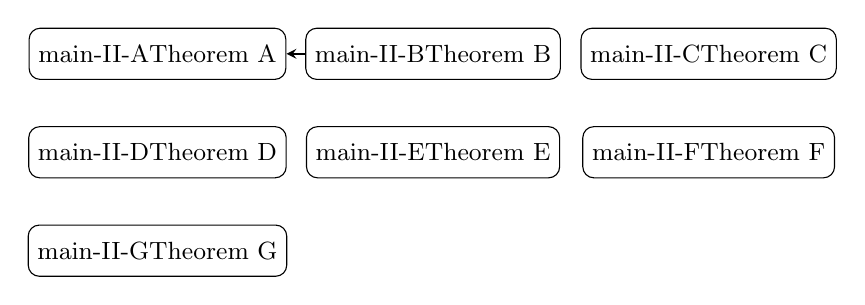
\begin{tikzpicture}[>=stealth,every node/.style={font=\small}]
\node[draw,rounded corners,minimum width=2.2cm,minimum height=.65cm] (TA) at (0.0,0.0) {\hyperlink{main-II-A}{Theorem A}};
\node[draw,rounded corners,minimum width=2.2cm,minimum height=.65cm] (TB) at (3.5,0.0) {\hyperlink{main-II-B}{Theorem B}};
\node[draw,rounded corners,minimum width=2.2cm,minimum height=.65cm] (TC) at (7.0,0.0) {\hyperlink{main-II-C}{Theorem C}};
\node[draw,rounded corners,minimum width=2.2cm,minimum height=.65cm] (TD) at (0.0,-1.25) {\hyperlink{main-II-D}{Theorem D}};
\node[draw,rounded corners,minimum width=2.2cm,minimum height=.65cm] (TE) at (3.5,-1.25) {\hyperlink{main-II-E}{Theorem E}};
\node[draw,rounded corners,minimum width=2.2cm,minimum height=.65cm] (TF) at (7.0,-1.25) {\hyperlink{main-II-F}{Theorem F}};
\node[draw,rounded corners,minimum width=2.2cm,minimum height=.65cm] (TG) at (0.0,-2.5) {\hyperlink{main-II-G}{Theorem G}};
\draw[->,semithick] (TB) to (TA);
\end{tikzpicture}
\caption{Reuse of the indicated body arguments among the main theorem groups.}
\par\medskip
\begingroup\small
\begin{tabularx}{\textwidth}{@{}p{.10\textwidth}X@{}}
\toprule Arrow & Supplying and receiving arguments\\\midrule
$B\to A$ & \SeriesRef{cdp:st:C.3.1} $\longrightarrow$ \SeriesRef{cdp:st:C4f}. The complete necessary smooth-fibre surface list is used in A.4.9 Step1 for twisted local-system cohomology. C4e Step1 uses C.3.1 plus the stated exclusion propositions to divide into the torus and h1(O)=1 branches; C4f Step2 explicitly applies that fixed-fibre persistence proof.\\
\bottomrule\end{tabularx}\endgroup\end{figure}

\clearpage
